\documentclass[letterpaper,10pt]{article}

\usepackage{enumitem}
\usepackage{titling}
\usepackage{listings,listings-rust}
\usepackage{url}
\usepackage{soul}
\usepackage{hyperref}
\usepackage{setspace}
\usepackage{subfig}
\usepackage{sectsty}
\usepackage{pdfpages}
\usepackage{colortbl}
\usepackage{multirow}
\usepackage{multicol}
\usepackage{relsize}
\usepackage{amsmath}
\usepackage{wasysym}
\usepackage{fancyvrb}
\usepackage[yyyymmdd]{datetime}
\usepackage{amsmath,amssymb,amsthm,graphicx,xspace}
\usepackage[titlenotnumbered,noend,noline]{algorithm2e}
\usepackage[compact]{titlesec}
\usepackage{XCharter}
\usepackage[T1]{fontenc}
\usepackage[scaled]{beramono}
\usepackage[normalem]{ulem}
\usepackage{booktabs}
\usepackage{tikz}
\usetikzlibrary{arrows.meta,automata,shapes,trees,matrix,chains,scopes,positioning,calc,decorations.pathreplacing}
\tikzstyle{block} = [rectangle, draw, fill=blue!20, 
    text width=2.5em, text centered, rounded corners, minimum height=2em]
\tikzstyle{bw} = [rectangle, draw, fill=blue!20, 
    text width=4em, text centered, rounded corners, minimum height=2em]

\definecolor{namerow}{cmyk}{.40,.40,.40,.40}
\definecolor{namecol}{cmyk}{.40,.40,.40,.40}
\renewcommand{\dateseparator}{-}

\let\LaTeXtitle\title
\renewcommand{\title}[1]{\LaTeXtitle{\textsf{#1}}}

\lstset{basicstyle=\footnotesize\ttfamily,breaklines=true}

\newcommand{\CPP}{C\nolinebreak\hspace{-.05em}\raisebox{.4ex}{\tiny\bf +}\nolinebreak\hspace{-.10em}\raisebox{.4ex}{\tiny\bf +}}
\def\CPP{{C\nolinebreak[4]\hspace{-.05em}\raisebox{.4ex}{\tiny\bf ++}}}

\newcommand{\handout}[5]{
  \noindent
  \begin{center}
  \framebox{
    \vbox{
      \hbox to 5.78in { {\bf ECE459: Programming for Performance } \hfill #2 }
      \vspace{4mm}
      \hbox to 5.78in { {\Large \hfill #4  \hfill} }
      \vspace{2mm}
      \hbox to 5.78in { {\em #3 \hfill \today} }
    }
  }
  \end{center}
  \vspace*{4mm}
}

\newcommand{\lecture}[3]{\handout{#1}{#2}{#3}{Lecture #1}}
\newcommand{\tuple}[1]{\ensuremath{\left\langle #1 \right\rangle}\xspace}

\addtolength{\oddsidemargin}{-1.000in}
\addtolength{\evensidemargin}{-0.500in}
\addtolength{\textwidth}{2.0in}
\addtolength{\topmargin}{-1.000in}
\addtolength{\textheight}{1.75in}
\addtolength{\parskip}{\baselineskip}
\setlength{\parindent}{0in}
\renewcommand{\baselinestretch}{1.5}
\newcommand{\term}{Winter 2023}

\singlespace


\begin{document}

\lecture{10 --- Software Architecture}{\term}{Jeff Zarnett}

\section*{System Design}
When you look at the situation, you might find the reason that the runtime of some code is what it is results from the design of the larger system in which the data lives. For example, if we have to do a lot of network calls to get the data that's needed, that will increase the time to do the operation compared to getting all the data locally or in only one network call. If we can't get all the data in one shot, we have to loop, and that loop might easily turn what is otherwise linear runtime into another of the accidentally-quadratic examples.

System design interviews are another popular screening method for candidates in industry. I [JZ] like this better than the leetcode interviews in terms of understanding a candidate's ability to do the (typical) work of software development. Unlike most algorithm implementations which are solved problems (that is, there exist one or more optimal answers), a lot of system design problems are quite open-ended and a problem that isn't ``read my mind'' likely has multiple valid options that you can choose... if you can justify your choice appropriately. I'll be happy to talk to you outside of class about my advice about how to approach this sort of interview.

Whether you can change the data layout or the system architecture is very situation-dependent. It is generally unlikely that you will be able to convince your company to split up their five-year old monolith codebase because it would be faster in some scenarios. It's not necessarily that your argument is invalid, it's just that the opportunity cost is huge and such a cost has to be outweighed by sufficient customer value. Similarly, it might be optimal for your use case to change how the data is represented in the database, but that version might be worse for another, more common, use case and so the right decision is leave it alone.

Sometimes you will get input, or get to make the choice. Let's talk about that a little bit!

\subsection*{Choosing the Right Architecture}

Software architecture courses cover this sort of topic in much more depth than this course has time for, but there is some time to think about the implications of architecture on the performance of the code. Most architecture decisions at the highest level -- like the level of monolith vs microservices -- are rarely made with performance in mind. We think about how best to represent the data or workflow... or what makes it easier for the developers to get work done. Alternatively, it's done with a wild guess about the performance situation: starting with microservices might be premised on the idea of scaling individual parts as needed sounds good but... will you really need it?

Since monoliths and microservices architecture have just been mentioned and will continue to feature in the rest of this topic, a quick explanation about these is warranted. A \textit{monolith} architecture is one in which there is one software project that contains the functionality. There can (and should) be module structure and some amount of organization in the system, but it's one deployable unit. Communication between different parts of the monolith are just in-memory or via some internal API. A \textit{microservices} architecture is one where there are many deployable units that work together via network communication. A medium-size or larger company almost certainly has some mixture of these things rather than a totally pure version of one of them. 

Which of these architectures is the best depends on the needs of the project. Monolith codebases were the standard for a long time, then microservices came into vogue, then there was a backlash, and the cycle goes on. My general advice on this would be to start with a monolith architecture and only start breaking things off to microservices if that proves to be valuable later.

\paragraph{Down a Level.} At the middle level, the decision of monolith or microservices is a given, but things like the design patterns come into play. Are we treating this as a producer-consumer problem? Blackboard-architecture? Message passing vs locking shared memory? Every approach has its pros and cons.

The discussing at this level is often around modelling the work to be done according to some convenient real-life analogy. Thinking of the processing of the data as an assembly line might be reasonable and a great way to make sure that the end result is correct. However, an implementation where the data moves from queue to queue could increase the overhead costs where the most efficient option is for a single thread to take the same work item through all steps. 

\paragraph{Implementation.} If we zoom in a bit more then we start to get into the implementation strategies for various parts of the system: do we have one thread? Spawn threads dynamically or use a thread pool? 

Maybe the framework you chose has made some of those decisions for you and you just get to choose the configuration parameters. Such as if your framework for responding to REST API calls uses a threadpool, but you get to choose the number of threads in the pool. There's some analysis to do there and you can start by thinking about how many CPUs are available and the nature of the tasks (i.e., do they get blocked frequently on I/O). With that said, more threads isn't always better due to overhead costs and communication costs. Ultimately, you will need to experiment and see what happens. In a later topic, we will discuss more about APIs and rate limits.


\paragraph{Complexity is the Enemy.}

The complexity that we create is often the result of looking to other companies -- particularly big companies that are leaders in the space -- and thinking that their choices are the reasons they are successful and that this is the new best practice and a ``silver bullet''\footnote{In folklore, silver is deadly to werewolves. A silver bullet is a metaphor for a simple solution that instantly solves a very big problem.}~\cite{architecture}. Looking at the industry leaders is instructive in many ways, but it's important to understand that many of their processes and choices are relevant for their size or scale and not for the rest of us. 

Some complexity is unavoidable as a result of making software used by real people to do their work. Tax software contains a huge number of rules and their exceptions because the tax code (based on law, regulations, etc) has so much inherent complexity. You can write to your government and ask them to simplify it, but unless they actually go through with it, you have to implement all the rules. The other kind of complexity, however, is the ones that software developers bring themselves with things like the factory pattern and \texttt{VisitationArrangingOfficer} classes. If you would like to lose some sanity, please enjoy \texttt{FizzBuzzEnterpriseEdition}: \url{https://github.com/EnterpriseQualityCoding/FizzBuzzEnterpriseEdition}
 
 
That's too much complexity on purpose, as some sort of parody of the excessive complexity that ``enterprise'' software has. Minimizing the non-essential complexity is important and it might sound like the advice is to not have abstraction, but we often talk about how abstraction reduces the complexity. Which is it?

Levels of abstraction are often perceived as a good thing in software architecture. They allow us to identify commonalities and de-duplicate code. In fact, there's a saying by David J. Wheeler that goes ``We can solve any problem by introducing an extra level of indirection.'' Wikipedia even calls it the Fundamental Theorem of Software Engineering. Mathematicians would hate this -- that's not a theorem, it's a pithy statement. Honestly, I [JZ] hate it too! Every layer of indirection can easily add additional overhead and result in duplication of work because the right information is not available. It also slows down the speed of development while you have to just write more stuff to move data around and to keep track of what should be on what level (and defend against degradation of the structure). Use as much abstraction as necessary and no more.

This is an ancient problem that has hopefully died out in years past, but companies sometimes had dedicated people working on architecture. They don't write code or actually implement anything. They are sometimes called ``architecture astronauts'' and they create, in the words of Joel Spolsky ``absurd, all-encompassing, high-level pictures of the universe that are all good and fine, but don’t actually mean anything at all.''~\cite{archastro}. Such a person usually does not do too much damage directly, but they encourage over-engineering and overly-complex solutions and either one can make your code slow!

How does over-architecting the code make the code slow? More services and more layers means more moving data around, and longer chains of communication are slower than shorter ones. How about some specifics?

\subsection*{Pitfalls}

Let us consider a few specific things that we could do wrong (and what to do about them). Just like the clickbait articles: four huge architecture mistakes to avoid! Number two will shock you! 

\paragraph{Excessive Network Calls.}
As previously referenced, reducing the number of network calls to get the data will be an improvement in the execution time. Network is slow and comes with unpredictable delays for various reasons. Each call has overhead to establish the connection, authenticate or validate the token\footnote{You \textit{are} including auth in your APIs, right? RIGHT?}, and unpack the request before any of the actual handling of it can take place. Thus, a lot of small requests is likely slower than one larger request. That may be partially offset by parallelization (like in asynchronous I/O situations), but not always.

The converse of that, though is that how much data is sent is also a factor in the length of time the communication takes. In a silly example, the app requests the whole table from the database server to the application and then searches and filters in memory. If the table is huge, sending all of it would take a long time. And that assumes that there's enough memory in the application and that the network call would not time out for being quite so large...

Worries about too many network calls can be used as an argument against a microservices architecture and favouring monoliths. It's a drawback of this architecture, to be sure, but it will never be the only criteria for deciding. Considering honestly the pros and cons of the architecture is normal, and if anyone ever tells you that their preferred solution has no drawbacks whatsoever, you should be very skeptical of that.

A common variant of this negative pattern is called the N+1 query problem. In short, it happens when you want to fetch a list of something, and then for each of those, fetch a list of related entities. Imagine you want to send e-mails to all the customers who have not yet paid their invoices. How to do that? Query for the customer ID of each invoices where the status is unpaid. Then, for each of those customer IDs, look up their e-mail address, and send the payment reminder e-mail to them.

At first glance that doesn't sound bad, because this is how you might carry out such an operation if doing it with printed paper invoices and contact info in your phone. But if there are 500 unpaid invoices, this approach results in 501 database queries. One to get the list of customer IDs, and then one each for every invoice to get the customer's e-mail. That's too many! 

You might think that such a thing is easy to avoid -- and it can be, if writing the SQL directly. We could use a join query to get the list of e-mails directly in one query, or use a \texttt{WHERE customer\_id IN (...)} type of clause to get it down to two queries. I prefer the one query approach, if possible, but two is certainly better than 500. What did I mean about not writing the SQL directly?

If you're using some sort of ORM (Object-Relational Mapping), then you have some intermediate framework (e.g., Hibernate, Rails ActiveRecord) that turns some (Rust or other language) code into some database query statements that you didn't write yourself. The ORMs may unintentionally generate for you the N+1 query-problem variant of your query. It's not on purpose, but it is worth checking the generated SQL these produce just to be sure. Some ORMs let you write your own SQL; for others you want to pursue strategies like eager loading (that is, fetching related entities alongside the ones you asked for originally, even if you might not need the related ones)~\cite{nplusone}. 

Here's an example of what an N+1 query looks like when you look at it with a profiler, from the Sentry Docs:\footnote{\url{https://docs.sentry.io/product/issues/issue-details/performance-issues/n-one-queries/}}
\begin{center}
  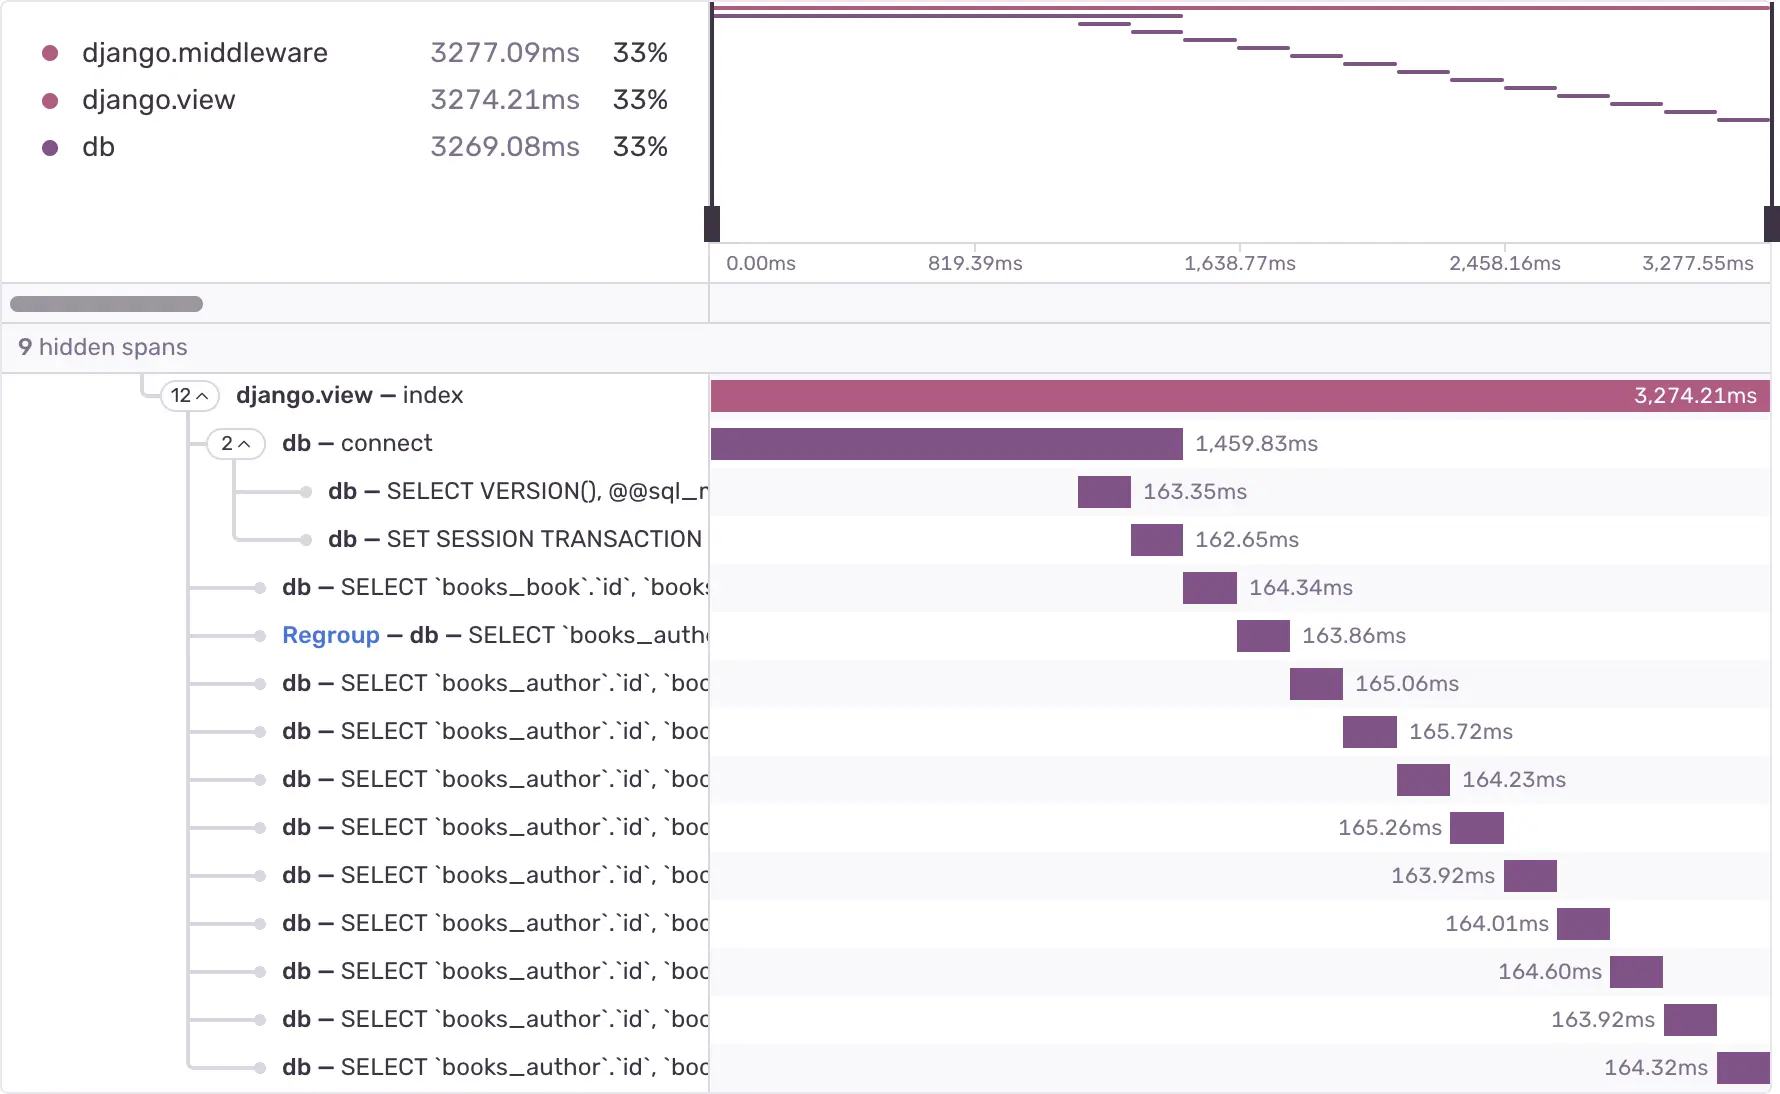
\includegraphics[width=0.7\textwidth]{images/nplusone.png}
\end{center}

The documentation for the Rust crate \texttt{juniper\_eager\_loading} provides a great example of how an N+1 query can result from a GraphQL schema. It builds on the Juniper package. We will not go too far into the details, but Juniper helps Rust backends use GraphQL.

In case you are not familiar with GraphQL, it is a data query language that lets the caller ask for the information that they want based on a known data schema. In a REST API, the verbs, endpoints, and the response shape are all determined by the implementer of the server responding. Perhaps the caller only wants to know the sum of unpaid invoice amount the account has, but if the API allows you only to get a list of unpaid invoices, you get back seven full invoices worth of data when all you cared about was the total field on that invoice. If you want to just ask about the total, well, add another endpoint... GraphQL is meant to avoid this by allowing you to ask just for what you need.

Okay, on to the example from the docs\footnote{\url{https://docs.rs/juniper-eager-loading/latest/juniper_eager_loading/index.html}} which, to give proper credit, are written by David Pedersen (\url{https://github.com/davidpdrsn/}) which I have modified a bit. Here's an example GraphQL schema:

\begin{lstlisting}
schema {
    query: Query
}

type Query {
    allUsers: [User!]!
}

type User {
    id: Int!
    country: Country!
}

type Country {
    id: Int!
    name: String!
}
\end{lstlisting}

And a caller executes the query:
\begin{lstlisting}
query SomeQuery {
    allUsers {
        country {
            name
        }
    }
}
\end{lstlisting}

The naive implementation will run the following queries:
\begin{lstlisting}
select * from users
select * from countries where id = ?
select * from countries where id = ?
select * from countries where id = ?
select * from countries where id = ?
...
\end{lstlisting}

But we actually would prefer...
\begin{lstlisting}
select * from users
select * from countries where id in (?, ?, ?, ?)
\end{lstlisting}

Sometimes we could solve this with eager loading, but that's harder in GraphQL since it's not possible to predict in advance which queries that callers will actually choose. Alright, how does this library work? The core idea is changing how the data structures work to load information if needed but avoid it if it's not. Let's look at the default way you might create a struct for \texttt{User} based on the schema above:

\begin{lstlisting}[language=Rust]
struct User {
    id: i32,
    country_id: i32
}
\end{lstlisting}
That's good, but the only way to get the name for a given country associated with users is to load the country itself from the database because the user only has the country's ID and not the name. Let's look at the source's alternative approach that separates the GraphQL model from the actual Rust structures.

\begin{lstlisting}[language=Rust]
mod models {
    pub struct User {
        id: i32,
        country_id: i32
    }

    pub struct Country {
        id: i32,
        name: String
    }
}

struct User {
    user: models::User,
    country: HasOne<Country>,
}

struct Country {
    country: models::Country
}

enum HasOne<T> {
    Loaded(T),
    NotLoaded,
}
\end{lstlisting}

With that, we can respond to the query in a more efficient way. First, load the users, get a list of country IDs, then query the countries in that set of IDs, and match them up. That means replacing the \texttt{User.country} value of \texttt{HasOne::NotLoaded} with \texttt{HasOne::Loaded(matching\_country)}. Then we can just return the set of names after the second query. A little bit of data modelling goes a long way here. This solution may not be the most optimal or the fewest lines of code, but it does demonstrate a big improvement over the naive version.


Finally, another strategy that helps reduce the number of network calls is caching. We've discussed it at great length earlier in the course, so no need to repeat any of that.

\paragraph{Bottlenecks (Chokepoints).} 

If your architecture results in repeatedly accessing the same data or same system, that can become a bottleneck on the way to completing work. One possible example of this that I [JZ] have seen is having an authorization service check the credentials on every API call internally in a microservices architecture. While that might be a good security policy to check every time, the communication costs in this scenario are high and it could end up overloading the authorization service (CPU) doing all the cryptographic calculations to check the credentials.

The solve for that particular problem is making it possible for a service to validate the credential without asking another system. A specific example of that is the \texttt{jwt} -- JSON web token -- which has some data (e.g., credentials) and is cryptographically signed with public-private key encryption so the server receiving the API call can check the credentials itself. Think of it as being like a passport: the government issues you the document and it has some security measures to prevent tampering; if you want to use your legitimate document to travel to another country the border control agents can validate the document without needing to do data exchange with the country that issued it. There are more levels at which the passport analogy for \texttt{jwt} works, but that's a digression.

The generalization of the solution above is to distribute the work to avoid the chokepoint: can other components take a part of it? Is the bottleneck part over-taking responsibility or would distributing it be putting work where it doesn't belong? That's worth considering.

\paragraph{Over-Taking Responsibility.}
The earlier example about searching and filtering in the application instead of the database also exemplifies another problem: over-taking responsibility. Even if the size of the table is so small that transmitting all of it over the network takes negligible time, why search and filter it in memory of the application? The database server has more information, like how the data is stored on disk or what index it can use to do the search. Therefore the most efficient approach is to let the DB do what it does best.

Another possibility is asking the backend system to do lots of work that would be better done in the frontend. Rendering the page in the backend may seem like a strange choice now, but it was the norm for a period of time. Moving that to the frontend or mobile app takes pressure off the backend.  This does not work for everything: remember that the backend should not trust any input from the frontend, so validation still needs to happen in the backend to be sure.

Over-taking responsibility is sometimes a result of organizational or technical constraints, such as gatekeeping or the remote server being run by another company. So the fastest, or only, way to accomplish what you want is to do it yourself, even if that's inefficient in execution. It's also possible to get in this situation because procurement (buying things or signing up for some external service) is too difficult and too slow: build vs buy decisions might always favour build if it means you can have something this month instead of next year. Over-taking responsibility also tends to result in more painful change management and high levels of tech debt if people are afraid of touching a critical and fragile system.

There are no software-architecture decisions that can solve organizational problems like this, but you can hopefully negotiate for what you want, or perhaps build some intermediary system that helps divide the workload rather than just suffering.



\paragraph{Too Much Waiting.} 
We've already covered asynchronous I/O, so at this point we are familiar with the idea that in some circumstances we can start an operation and not wait for the results before starting the next. We know that eliminates unnecessary waits and there's even a potential benefit of multiple I/O requests executing in parallel to bring down completion time. Still, there's more to explore on this idea.

Moving to an asynchronous model is also valuable in reducing \textit{perceived} waits even if the actual execution time is no faster. Remember from a previous operating systems course the concept of \textit{response time}. This is the time that it takes to get some result back. Emphasis on the word some in that sentence. The user has a better experience if we start returning partial results sooner and then load the rest later. How many websites have you been to where the page loads but different panels have the spinning loader while other stuff comes in? 


The last way in which we can end up with too much waiting is every thread or process waiting to acquire a lock around some shared data. Imagine there is one \texttt{Arc<Mutex<Vector>{}>} and every thread wants to add data to it. We can make that much more efficient if we have one thread that owns the data and the other threads send their data via a channel or other message-passing mechanism to the owning thread and the owning thread takes those and processes them in turn. Is there overhead in establishing the channel and sending/receiving the data? Sure, but it is offset by reducing (eliminating) lock contention around the vector. Actually, let's talk some more in the next topic about the proper use of locks and the concept of lock contention. 

\input{bibliography.tex}

\end{document}
